\documentclass{article}


\usepackage{amsmath}
\usepackage{tikz}
\usepackage{float}
\usepackage{geometry}
\usepackage{setspace}
\usepackage{cancel}

\geometry{margin=0.8in}
\title{\bfseries CHEG231 exam 1 sheet}
\author{kyle wodehouse}

\begin{document}
\maketitle

\subsection*{mass balances}
\[ \Delta M = \Delta M_{\text{in}} - \Delta M_{\text{out}} \hspace{5em} \frac{dM}{dt} = \dot{M_{\text{in}}} - \dot{M_{\text{out}}} \]
\subsection*{energy balance, difference form}
\[ \left[ U + m \left( \frac{v^2}{2} + gh \right) \right]_f - \left[ U + m \left( \frac{v^2}{2} + gh \right) \right]_i = Q + W_S + W_{PV} \ldots + \sum_{k=1}^{K} \Delta m_k \left( \hat{U} + P\hat{V} + \frac{v^2}{2} + gh \right)_k \]
\subsection*{energy balance, differential form}
\[ \frac{d}{dt} \left\{ U + M\left( \frac{v^2}{2} + mg\right) \right\} = \dot{Q} + \dot{W_s} + \dot{W_{PV}} + \sum_{k=1}^{K} \dot{m_k} \left( \hat{U} + P\hat{V} + \frac{v^2}{2} + mg \right) \]
\subsection*{entropy balances}
\[ S_2 - S_1 = \sum_{k} \int_{t_1}^{t_2} \dot{m}_k \hat{S}_k \ dt + \int_{t_1}^{t_2} \frac{\dot{Q}}{T} \ dt + S_{\text{gen}} \hspace{5em} \frac{dS}{dt} = \sum_{k=1}^{K} \dot{m}_k \hat{S}_k + \frac{\dot{Q}}{T} + \dot{S}_{\text{gen}} \]

\hrule


\begin{table}[H]
    \centering
    \doublespacing
    \begin{tabular}{cc}
        \( C_V = \left(\frac{\partial \underbar{U}}{\partial T}\right)_V \) & \( C_P = \left(\frac{\partial \underbar{H}}{\partial T}\right)_P \)\\
        For Ideal Gasses: $C_P^* = C_V^* + R$ & and $C_V^*  = df/2$ \\
        $\underbar{U}^{IG} = C_V^* T$ & $\underbar{H}^{IG} = C_P^* T$
    \end{tabular}
    \begin{tabular}{cc}
    \end{tabular}
\end{table}

For solids and liquids: $\underbar{H} \approx \underbar{U}$ and incompressible. Also $C_{\text{P}} = 3NR = 24.924$ J/mol*K approx for solids.

\section*{lever rule (properties of one component system w/ two phases)}
\[ \hat{\theta} = \omega^I \hat{\theta}^I + \omega^{II}\hat{\theta}^{II} = \omega^I \hat{\theta}^I + (1 - \omega^I)\hat{\theta}^{II} \]

\section*{entropy stuff}
\[
    \Delta \underbar{S}_{\text{ideal gas}} = C_p^* \ln \left( \frac{T_2}{T_1} \right) - R \ln \left( \frac{P_2}{P_1} \right)
\]
\[
    \Delta \underbar{S}_{\text{Liquid}} = C_p^* \ln \left( \frac{T_2}{T_1} \right) 
\]

Helmholts Energy: difference is work required to bring closed, isothermal, constant volume system from state 1 to state 1
\[ A = U - TS\]
Gibbs energy: helpmholtz but for closed, isothermal, isobaric system
\[ G = U + PV - TS = H - TS\]
Gibbs equation
\[ d\underbar{$U$} = T\,d\underbar{$S$} - P\,d\underbar{$V$}\]

\section{Carnot Derivation}
Consider a closed system of a heat engine
\begin{center}
    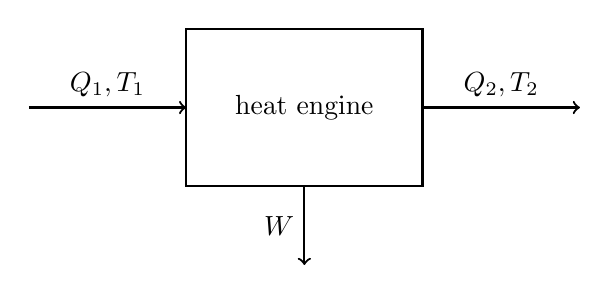
\begin{tikzpicture}
        \draw[thick] (0,0) rectangle (3,2) node[midway] {heat engine};
        
        \draw[->, thick] (-2,1) -- (0,1) node[midway, above] {$Q_1, T_1$};
        \draw[->, thick] (3,1) -- (5,1) node[midway, above] {$Q_2, T_2$};
        \draw[->, thick] (1.5,0) -- (1.5,-1) node[midway, left] {$W$};
    \end{tikzpicture}
\end{center}
energy balance:
\[ \cancel{\frac{dU}{dt}} = \dot{Q} + \dot{W} + \cancel{\sum \dot{m}_k()_k} \]
\[ 0 = Q_1 + Q_2 + W\]

entropy balance:
\[ \cancel{\frac{dS}{dt}} = \frac{\dot{Q}_1}{T_1} + \frac{\dot{Q}_2}{T_2} + \cancel{\sum_{k=1}^{K}\dot{m}_k \hat{S}_k} + \dot{S}_{\text{gen}} \]
\[ 0 = \frac{\dot{Q}_1}{T_1} + \frac{\dot{Q}_2}{T_2}  + \dot{S}_{\text{gen}} \]
integrating, and remembering that reversible processes are more efficient than irreversible processes
\[ 0 = \frac{Q_1}{T_1} + \frac{Q_2}{T_2} \]
\[ \frac{Q_1}{T_1} = \frac{- Q_2}{T_2} \]
\[ Q_2 = \frac{- Q_1 T_2}{T_1} \]
and taking this into the energy balance
\[ -W = Q_1 + \frac{- Q_1 T_2}{T_1} = Q_1 \left(\frac{T_1 - T_2}{T_1}\right) \]
\[ \eta = \frac{-W}{Q_1} = \left(\frac{T_1 - T_2}{T_1}\right) \]



\end{document}